% Options for packages loaded elsewhere
\PassOptionsToPackage{unicode}{hyperref}
\PassOptionsToPackage{hyphens}{url}
%
\documentclass[
  12pt,
]{report}
\usepackage{lmodern}
\usepackage{setspace}
\usepackage{amssymb,amsmath}
\usepackage{ifxetex,ifluatex}
\ifnum 0\ifxetex 1\fi\ifluatex 1\fi=0 % if pdftex
  \usepackage[T1]{fontenc}
  \usepackage[utf8]{inputenc}
  \usepackage{textcomp} % provide euro and other symbols
\else % if luatex or xetex
  \usepackage{unicode-math}
  \defaultfontfeatures{Scale=MatchLowercase}
  \defaultfontfeatures[\rmfamily]{Ligatures=TeX,Scale=1}
\fi
% Use upquote if available, for straight quotes in verbatim environments
\IfFileExists{upquote.sty}{\usepackage{upquote}}{}
\IfFileExists{microtype.sty}{% use microtype if available
  \usepackage[]{microtype}
  \UseMicrotypeSet[protrusion]{basicmath} % disable protrusion for tt fonts
}{}
\makeatletter
\@ifundefined{KOMAClassName}{% if non-KOMA class
  \IfFileExists{parskip.sty}{%
    \usepackage{parskip}
  }{% else
    \setlength{\parindent}{0pt}
    \setlength{\parskip}{6pt plus 2pt minus 1pt}}
}{% if KOMA class
  \KOMAoptions{parskip=half}}
\makeatother
\usepackage{xcolor}
\IfFileExists{xurl.sty}{\usepackage{xurl}}{} % add URL line breaks if available
\IfFileExists{bookmark.sty}{\usepackage{bookmark}}{\usepackage{hyperref}}
\hypersetup{
  pdftitle={Núcleo de Estudos em Representação e Democracia},
  hidelinks,
  pdfcreator={LaTeX via pandoc}}
\urlstyle{same} % disable monospaced font for URLs
\usepackage[left=3cm,right=3cm,top=2cm,bottom=2cm]{geometry}
\usepackage{graphicx,grffile}
\makeatletter
\def\maxwidth{\ifdim\Gin@nat@width>\linewidth\linewidth\else\Gin@nat@width\fi}
\def\maxheight{\ifdim\Gin@nat@height>\textheight\textheight\else\Gin@nat@height\fi}
\makeatother
% Scale images if necessary, so that they will not overflow the page
% margins by default, and it is still possible to overwrite the defaults
% using explicit options in \includegraphics[width, height, ...]{}
\setkeys{Gin}{width=\maxwidth,height=\maxheight,keepaspectratio}
% Set default figure placement to htbp
\makeatletter
\def\fps@figure{htbp}
\makeatother
\setlength{\emergencystretch}{3em} % prevent overfull lines
\providecommand{\tightlist}{%
  \setlength{\itemsep}{0pt}\setlength{\parskip}{0pt}}
\setcounter{secnumdepth}{-\maxdimen} % remove section numbering
\renewcommand{\contentsname}{Sumário}
\usepackage{float}
\floatplacement{figure}{H}

\title{Núcleo de Estudos em Representação e Democracia}
\usepackage{etoolbox}
\makeatletter
\providecommand{\subtitle}[1]{% add subtitle to \maketitle
  \apptocmd{\@title}{\par {\large #1 \par}}{}{}
}
\makeatother
\subtitle{NERD}
\author{}
\date{\vspace{-2.5em}}

\begin{document}
\maketitle

{
\setcounter{tocdepth}{1}
\tableofcontents
}
\setstretch{1.5}
\pagebreak

\hypertarget{apresentauxe7uxe3o}{%
\section{1. Apresentação}\label{apresentauxe7uxe3o}}

O Núcleo de Estudos em Representação e Democracia -- NERD -- se
configura como um grupo de pesquisa que reúne pesquisadores de Ciência
Política, Sociologia e Administração pública de instituições ligadas ao
Programa de pós-graduação em Sociologia Política da UENF. Está integrado
aos cursos de graduação do Centro de Ciências do Homem - CCH - e
vinculado ao Laboratório de Estudos da Sociedade Civil e do Estado
(LESCE).

O grupo de pesquisa aborda a interseção entre três grandes dimensões da
análise de sistemas políticos democráticos: governos locais,
comportamento eleitoral e partidos políticos. A partir dos estudos sobre
comportamento dos eleitores pretende-se integrar os achados empíricos às
teorias sobre estratégias dos partidos políticos nas administrações
públicas subnacionais, assim como interagir com análises sobre reeleição
de prefeitos, análises que abordam ideologia partidária e gastos
públicos no Brasil.

O NERD busca abranger estudos sobre política nacional visando estudos e
análises comparadas. As atividades do NERD procuram atender a demanda de
informações e análises no Brasil, assim como da interação da dimensão
política com o desenvolvimento socioeconômico.

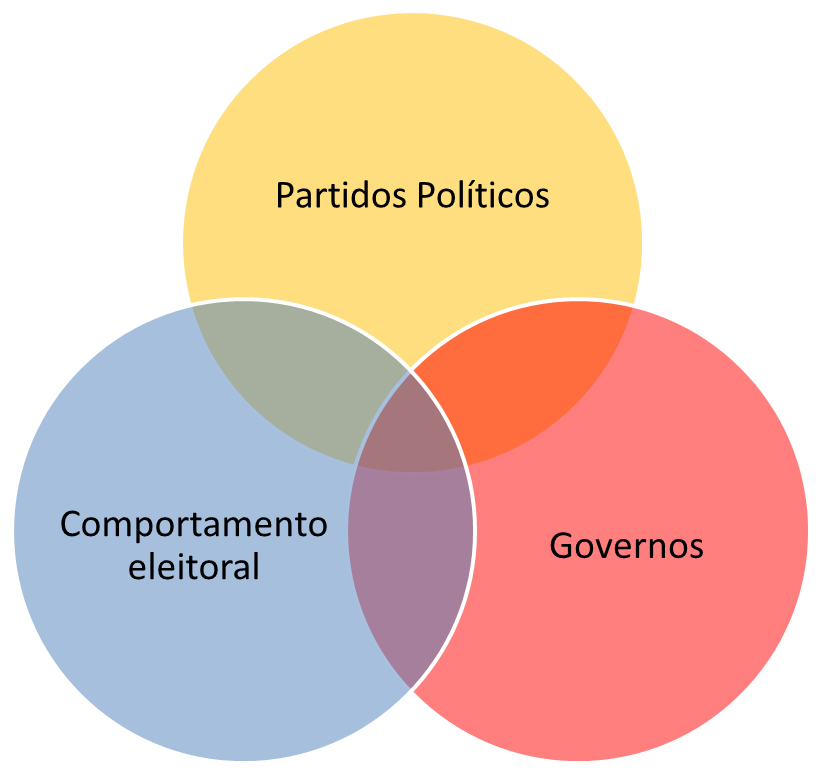
\includegraphics{nerd_diagrama_venn.png}

O núcleo teve início da suas atividades com o projeto de pesquisa
``Competição Eleitoral nos Municípios Brasileiros'', em 2011, deu
sequencia com o projeto CNPq ``Poder Local, Partidos políticos e
eleições municipais no Brasil pós 1988'', e atualmente é financiado pela
FAPERJ com projeto ``Petro rendas e política local: competição eleitoral
e políticas públicas em municípios produtores de petróleo''.

O NERD tem por filosofia a utilização de softwares livres e preza pela
divulgação de resultados científicos com reprodutibilidade.

\hypertarget{justificativa}{%
\section{2. Justificativa}\label{justificativa}}

A formação do núcleo de pesquisa se justifica pela necessidade de
reunir, coordenar e estimular pesquisadores que coadunam interesses
temáticos com a unidade teórico-metodológica sob o mesmo guarda-chuva
institucional.

A maioria dos trabalhos que abordam o tema da política municipal
analisam as capitais estaduais ou municípios que introduziram novas
formas de participação, como o orçamento participativo e os conselhos
municipais, em geral, por meio de metodologias qualitativas que
privilegiam os estudos de casos. Na intenção de atenuar esse déficit, o
Núcleo de Estudos em Representação e Democracia -- NERD prioriza
abordagens quantitativas que abarcam as 5.570 unidades federativas.

A Constituição de 1988 se orienta claramente por um princípio
descentralizador e municipalista. No Capítulo IV (``Dos Municípios''),
artigo 29 se estabelece que ``o município reger-se-á por lei orgânica,
votada em dois turnos, com interstício mínimo de dez dias, e aprovada
por dois terços da Câmara Municipal (\ldots)''. Já no artigo 30 do mesmo
capítulo se estabelecem as competências dos municípios, em que se
destacam as áreas de educação pré-escolar, ensino fundamental, saúde e
saneamento, podendo ser solicitado para o cumprimento dessas funções, a
cooperação técnica e financeira do Estado e da União. Incumbe também aos
governos municipais instituir e arrecadar os tributos correspondentes a
suas competências, assim como a alocação das receitas.

Junto com o incremento da autonomia municipal e de suas atribuições nas
áreas mencionadas, a Constituição também valorizou os legislativos
municipais, outorgando-lhes a possibilidade de introduzir emendas ao
orçamento municipal, reforçando o poder político das Câmaras de
Vereadores. Além dessa nova potestade, a relevância desses órgãos radica
não somente na visibilidade dos temas sobre os que devem legislar muito
próximos da vida cotidiana dos cidadãos, mas também, no vínculo direto
de seus membros com as bases eleitorais. Porém, vários trabalhos têm
destacado a hipertrofia dos Executivos nos municípios pequenos e médios,
em relação aos Legislativos e Judiciários (Abrucio, 1994; Nunes, 1991).

Concomitantemente ao aumento das responsabilidades e atribuições dos
municípios, houve também, a partir da aprovação da nova Constituição, um
aumento das fontes tributárias e um repasse automático de receitas por
parte dos Estados e do Governo Federal. Com efeito, as principais
consequências da reforma constitucional foram um aumento substancial do
poder tributário dos governos subnacionais nas suas respectivas
jurisdições e um incremento das transferências da União para Estados e
municípios (Abrucio e Couto, 1996; Giambiagi, 1991).

Os dados censitários a partir de 1991 indicaram um crescimento
populacional mais acelerado dos municípios de pequeno, médio e grande
porte. Ressalta-se que em alguns municípios de grande porte tal
perspectiva se manifestava com um ritmo de crescimento populacional
superior ao das Regiões Metropolitanas na década de 1970. Nestes termos,
Baeninger (1999: p.538), aponta para o fato de que ``os municípios
não-metropolitanos registraram um incremento relativo de 22\%, no
período 1970-1980, e de 6,7\% no de 1991-1996''. Assim, pode-se perceber
que o processo de interiorização que já vinha ocorrendo no Brasil em
décadas anteriores, continuou sendo observado, agudizando-se a partir
dos anos 2000.

Outro ponto relevante é o fato de haver uma defasagem no que se refere
as análises que se pretendem a compreender os possíveis efeitos causais
entre a discricionariedade do ocupante da cadeira do executivo local e a
provisão de políticas públicas.

Uma das maiores consequências da descentralização federativa foi o
destaque dado aos governos locais no que tange à provisão de políticas
sociais, como as políticas de saúde e as políticas de educação. A
despeito dos mínimos constitucionais de aplicação financeira nessas
áreas, estudos apontam que ainda há espaço para que os prefeitos ponham
as suas marcas políticas na gestão dessas ações estatais. Estudar este
aspecto é um dos comprometimentos do laboratório.

Ainda nesse contexto, as pesquisas empíricas realizadas pelo NERD
pretendem dar conta das relações entre as práticas enquanto gestor
municipal e a premiação ou punição eleitoral. Um dos encargos
científicos deste grupo é analisar os possíveis impactos da gestão da
máquina municipal sobre o fracasso ou sucesso eleitoral dos prefeitos,
tais como o aumento/diminuição do gasto com educação, aumento/diminuição
de leitos hospitalares.

Com base nestas considerações propõe-se um núcleo de pesquisa que
privilegia as questões relativas à política pública, eleições e ao
desenvolvimento socioeconômico. As atividades do núcleo podem ser
agrupadas em três grandes eixos analíticos: (1) o funcionamento das
instituições políticas (eleições, administração pública, comportamento
parlamentar e relação executivo-legislativo); (2) desenvolvimento
socioeconômico (atividades produtivas, estrutura social, mercado de
trabalho e perfil social dos municípios); (3) comportamento eleitoral e
opinião pública.

\hypertarget{objetivos}{%
\section{3. Objetivos}\label{objetivos}}

Os projetos de pesquisa e nas suas atividades em geral, analisar as
possíveis relações entre trÊs eixos temáticos: o comportamento eleitoral
do brasileiro, estratégias eleitorais partidárias e a provisão de
políticas públicas locais.

No que concerne ao comportamento eleitoral, o NERD tem por objetivo
construir análises no nível individual sobre um conjunto de variáveis
atitudinais e comportamentais que englobam apoio à democracia,
tolerância política, intenção de voto, ideologia, conservadorismo,
partidarismo, etc.

Na dimensão das estratégias eleitorais dos partidos políticos, o grupo
de pesquisa desenvolve uma série de estudos acerca dos desempenhos
eleitorais, lançamentos de candidaturas, competição intra e inter
partidárias, organização interna dos partidos, políticas eleitorais de
gênero, assim como instituições reguladoras das eleições, como TRE's e
TSE.

Na dimensão sobre governos locais, inclui-se o intuito de contribuir com
produção de informação e conhecimento científico relevante sobre o
desenvolvimento político, econômico e social dos municípios brasileiros,
assim como estudos que abordem o desempenho político institucional de
outras regiões e municípios do país, possibilitando ainda a realização
de análises comparadas. Portanto, o NERD tem também por objetivo
promover pesquisas sobre a evolução política e eleitoral no nível
municipal.

Os objetivos específicos do núcleo a destacar são:

\begin{itemize}
\item
  Difusão dos resultados das pesquisas para o âmbito acadêmico e
  extra-acadêmico (encontros, seminários, mini-cursos, etc.).
\item
  Promover a participação de alunos de graduação (iniciação científica)
  e pós-graduação nas atividades do núcleo.
\item
  Organizar e compartilhar bases de dados destinados a subsidiar
  pesquisas acadêmicas e a demandas de instituições públicas e privadas,
  formadores de opinião e público em geral.
\item
  Participar em editais de financiamento de pesquisas e atividades de
  extensão.
\item
  Receber pesquisadores de outras instituições.
\item
  Promover pesquisas interinstitucionais com pesquisadores nacionais e
  internacionais.
\end{itemize}

\hypertarget{membros}{%
\section{4. Membros}\label{membros}}

\href{http://lattes.cnpq.br/4676437210734787}{Vitor de Moraes Peixoto}
\hfill\break \textbf{Coordenador} \hfill\break Professor Associado
\hfill\break Universidade Estadual do Norte Fluminense Darcy Ribeiro
\hfill\break Centro de Ciências do Homem \hfill\break Laboratório de
Estudos da Sociedade Civil e do Estado \hfill\break E-mail:
\href{mailto:vpeixoto@pq.uenf.br}{\nolinkurl{vpeixoto@pq.uenf.br}}
\hfill\break

\href{http://lattes.cnpq.br/4208615645719699}{Renato Barreto de Souza}
\hfill\break Professor do Instituto Federal Fluminense \hfill\break Pós
doutorando do Programa de Pós-Graduação em Sociologia Politica
\hfill\break Universidade Estadual do Norte Fluminense Darcy Ribeiro
\hfill\break Laboratório de Estudos do Estado e da Sociedade Civil
\hfill\break E-mail:
\href{mailto:renatobs@gmail.com}{\nolinkurl{renatobs@gmail.com}}
\hfill\break

\href{http://lattes.cnpq.br/9603711186053943}{Cleinton Roberto Perpeto
de Souza}\hfill\break Pós doutorando do Programa de Pós-Graduação em
Sociologia Politica \hfill\break Universidade Estadual do Norte
Fluminense Darcy Ribeiro \hfill\break Laboratório de Estudos do Estado e
da Sociedade Civil \hfill\break E-mail:
\href{mailto:cleintongael@gmail.com}{\nolinkurl{cleintongael@gmail.com}}
\hfill\break

\href{http://lattes.cnpq.br/6620703529177610}{Patricia de Oliveira
Burlamaqui}\hfill\break Pós doutoranda do Programa de Pós-Graduação em
Sociologia Politica \hfill\break Universidade Estadual do Norte
Fluminense Darcy Ribeiro \hfill\break Laboratório de Estudos do Estado e
da Sociedade Civil \hfill\break E-mail:
\href{mailto:pburlamaqui@gmail.com}{\nolinkurl{pburlamaqui@gmail.com}}
\hfill\break

\href{http://lattes.cnpq.br/7250750885312461}{Ralph André Crespo}
\hfill\break Doutorando do Programa de Pós-Graduação em Sociologia
Politica \hfill\break Universidade Estadual do Norte Fluminense Darcy
Ribeiro \hfill\break Laboratório de Estudos do Estado e da Sociedade
Civil \hfill\break E-mail:
\href{mailto:ralph.crespo@pq.uenf.br}{\nolinkurl{ralph.crespo@pq.uenf.br}}
\hfill\break

\href{http://lattes.cnpq.br/1477388811747167}{Jheniffer Vieira de
Almeida} \hfill\break Doutoranda do Programa de Pós-Graduação em
Sociologia Politica \hfill\break Universidade Estadual do Norte
Fluminense Darcy Ribeiro \hfill\break Laboratório de Estudos do Estado e
da Sociedade Civil \hfill\break E-mail:
\href{mailto:jhenifferalmeida@pq.uenf}{\nolinkurl{jhenifferalmeida@pq.uenf}}
\hfill\break

\href{http://lattes.cnpq.br/9433034841064768}{Raphael de Mello Veloso}
\hfill\break Doutorando do Programa de Pós-Graduação em Sociologia
Politica \hfill\break Universidade Estadual do Norte Fluminense Darcy
Ribeiro \hfill\break Laboratório de Estudos do Estado e da Sociedade
Civil \hfill\break E-mail:
\href{mailto:raphamv@gmail.com}{\nolinkurl{raphamv@gmail.com}}
\hfill\break

\href{http://lattes.cnpq.br/1675744772217864}{Gisele Braga Bastos}
\hfill\break Doutoranda do Programa de Pós-Graduação em Sociologia
Politica \hfill\break Universidade Estadual do Norte Fluminense Darcy
Ribeiro \hfill\break Laboratório de Estudos do Estado e da Sociedade
Civil \hfill\break E-mail:
\href{mailto:gibragabastos@pq.uenf.br}{\nolinkurl{gibragabastos@pq.uenf.br}}
\hfill\break

\href{http://lattes.cnpq.br/6717255818088404}{Jessica Matheus de Souza}
\hfill\break Doutoranda do Programa de Pós-Graduação em Sociologia
Politica \hfill\break Universidade Estadual do Norte Fluminense Darcy
Ribeiro \hfill\break Laboratório de Estudos do Estado e da Sociedade
Civil \hfill\break E-mail:
\href{mailto:jessicamatheus@pq.uenf.br}{\nolinkurl{jessicamatheus@pq.uenf.br}}
\hfill\break

\href{http://lattes.cnpq.br/8178088513307546}{Wallace da Silva Mello}
\hfill\break Doutorando do Programa de Pós-Graduação em Sociologia
Politica \hfill\break Universidade Estadual do Norte Fluminense Darcy
Ribeiro \hfill\break Laboratório de Estudos do Estado e da Sociedade
Civil \hfill\break E-mail:
\href{mailto:wallacesilvamello@pq.uenf.br}{\nolinkurl{wallacesilvamello@pq.uenf.br}}
\hfill\break

\href{http://lattes.cnpq.br/5038496684551538}{Thiago Pimentel Soares}
\hfill\break Mestrando do Programa de Pós-Graduação em Sociologia
Politica \hfill\break Universidade Estadual do Norte Fluminense Darcy
Ribeiro \hfill\break Laboratório de Estudos do Estado e da Sociedade
Civil \hfill\break E-mail:
\href{mailto:tpsoares@hotmail.com}{\nolinkurl{tpsoares@hotmail.com}}
\hfill\break

\href{http://lattes.cnpq.br/6781198318316057}{Rafael Soares Salles}
\hfill\break Mestrando do Programa de Pós-Graduação em Sociologia
Politica \hfill\break Universidade Estadual do Norte Fluminense Darcy
Ribeiro \hfill\break Laboratório de Estudos do Estado e da Sociedade
Civil \hfill\break  E-mail:
\href{mailto:rafael.salles@pq.uenf.br}{\nolinkurl{rafael.salles@pq.uenf.br}}
\hfill\break

\href{http://lattes.cnpq.br/9277299850069272}{João Gabriel Ribeiro
Pessanha Leal} \hfill\break Mestrando do Programa de Pós-Graduação em
Ciência Política \hfill\break Universidade Federal do Estado do Rio de
Janeiro \hfill\break E-mail:
\href{mailto:joaoleal@pq.uenf.br}{\nolinkurl{joaoleal@pq.uenf.br}}
\hfill\break

\href{http://lattes.cnpq.br/8424422005329610}{Larissa Martins Marques}
\hfill\break Graduanda do Curso de Administração Pública \hfill\break
Universidade Estadual do Norte Fluminense Darcy Ribeiro \hfill\break
Laboratório de Estudos do Estado e da Sociedade Civil \hfill\break
E-mail:
\href{mailto:larissamarques@pq.uenf.br}{\nolinkurl{larissamarques@pq.uenf.br}}
\hfill\break

\href{http://lattes.cnpq.br/6781198318316057}{Matheus Virginio Harduim
Machado} \hfill\break Graduando do Curso de Ciências Sociais
\hfill\break niversidade Estadual do Norte Fluminense Darcy Ribeiro
\hfill\break Laboratório de Estudos do Estado e da Sociedade Civil
\hfill\break E-mail:
\href{mailto:m.harduim@pq.uenf.br}{\nolinkurl{m.harduim@pq.uenf.br}}
\hfill\break

\href{http://lattes.cnpq.br/7181203038300743}{Fernanda da Silva Souza}
\hfill\break Graduanda do Curso de Ciências Sociais \hfill\break
niversidade Estadual do Norte Fluminense Darcy Ribeiro \hfill\break
Laboratório de Estudos do Estado e da Sociedade Civil \hfill\break
E-mail:
\href{mailto:fer.souzaa1@outlook.com}{\nolinkurl{fer.souzaa1@outlook.com}}
\hfill\break

\href{http://lattes.cnpq.br/6943283489647623}{Lara Bernardo de Oliveira}
\hfill\break Graduanda do Curso de Ciências Sociais \hfill\break 
niversidade Estadual do Norte Fluminense Darcy Ribeiro \hfill\break
Laboratório de Estudos do Estado e da Sociedade Civil \hfill\break
E-mail:
\href{mailto:lalabernardo1904@gmail.com}{\nolinkurl{lalabernardo1904@gmail.com}}
\hfill\break

\href{http://lattes.cnpq.br/5081047341028478}{Paula Regis Cordeiro de
Araujo} \hfill\break Graduanda do Curso de Administração Pública
\hfill\break Universidade Estadual do Norte Fluminense Darcy Ribeiro
\hfill\break Laboratório de Estudos do Estado e da Sociedade Civil
\hfill\break E-mail:
\href{mailto:regispaularegis@gmail.com}{\nolinkurl{regispaularegis@gmail.com}}
\hfill\break

\hypertarget{projetos}{%
\section{5. Projetos}\label{projetos}}

\hypertarget{em-execuuxe7uxe3o}{%
\subsection{5.1 - Em execução:}\label{em-execuuxe7uxe3o}}

\textbf{Economia social da (In)tolerância política: como avaliações da
economia, mobilidade social, escolaridade, gênero e religião impactam as
atitudes democráticas no Brasil contemporâneo}

Este projeto visa produzir análises acerca das avaliações e percepções
econômicas e seus impactos sobre um conjunto de atitudes e
comportamentos individuais conhecidos por tolerância política ao longo
dos últimos quatro ciclos eleitorais. Além disso, busca compreender como
as variáveis sociológicas clássicas tais como religião, escolaridade,
renda e sexo se relacionam aos aspectos tolerância e apoio à democracia.
Dessa forma, procura aferir como essas variáveis interferem na opinião
pública sobre a democracia, investigando e diferenciando o comportamento
de grupos específicos em relação as organizações democráticas.

Fomento: UENF-Faperj

\textbf{Petro rendas e política local: competição eleitoral e políticas
públicas em municípios produtores de petróleo}

Este projeto de pesquisa tem como objetivo a investigação de padrões
partidários de gastos públicos em municípios petro-rentistas em dois
contextos econômicos: de abundancias e crises severas de recursos.
Propõem-se construir indicadores e testar modelos econométricos
multivariados no intuito de explorar as características políticas dos
executivos municipais que estão associadas à variação de padrões de
comportamentos orçamentários na administração de recursos
indenizatórios. Buscar-se-á comparar unidades da federação com
características sociodemográficas similares no intuito de testar
hipóteses os efeitos dos recursos dos royalties e participações
especiais nos padrões de gastos sociais e com maquina pública dos
partidos políticos.

Fomento: FAPERJ - APQ1 CNPq - UENF

\hypertarget{projetos-finalizados}{%
\subsection{5.2 - Projetos finalizados:}\label{projetos-finalizados}}

\begin{itemize}
\item
  Projeto FAPERJ E-26/111-677/2011.``Competição Eleitoral nos Municípios
  Brasileiros''.
\item
  Projeto CNPq: ``Poder local, Partidos políticos e eleições municipais
  no Brasil pós 1988''.
\item
  Projeto FAPERJ APQ3 E-26/112.214/2013. ``Financiamento de campanhas
  eleitorais no Brasil''.
\end{itemize}

\hypertarget{localizauxe7uxe3o}{%
\section{6. Localização}\label{localizauxe7uxe3o}}

Universidade Estadual do Norte Fluminense Darcy Ribeiro \hfill\break
Centro de Ciências do Homem -- CCH -- Sala 108 - B \hfill\break Av.
Alberto Lamego, 2000 - Parque Califórnia \hfill\break Campos dos
Goytacazes - RJ \hfill\break CEP: 28013-602 \hfill\break Tel: 22
27397040 \hfill\break

\href{https://www.google.com.br/maps/place/Av.+Alberto+Lamego,+2000+-+Parque+California,+Campos+dos+Goytacazes+-+RJ,+28013-602/@-21.7618032,-41.2934395,18z/data=!4m5!3m4!1s0xbdd59a0a81985b:0xf4793c8dba9348ac!8m2!3d-21.7623551!4d-41.2946988}{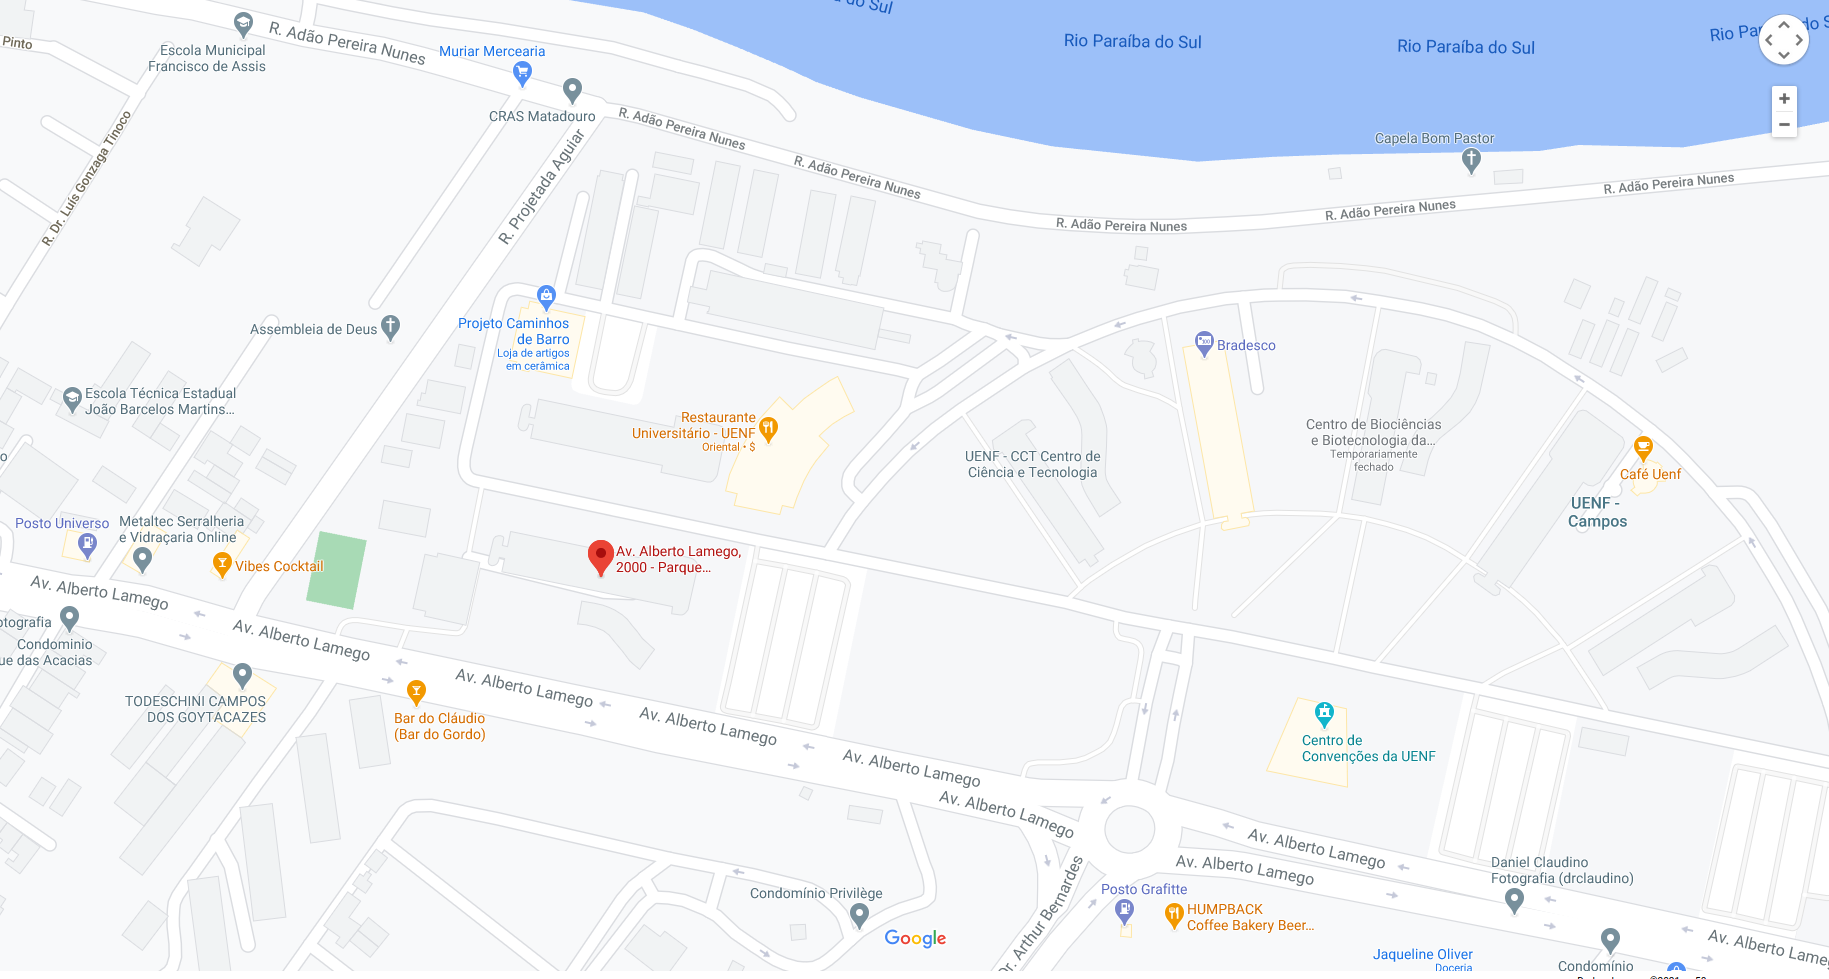
\includegraphics{mapa.png}}

\end{document}
